%------------------------------------------------
% E_8
%------------------------------------------------
\begin{figure} \label{fig:E8Dynkindiagram}
\centering
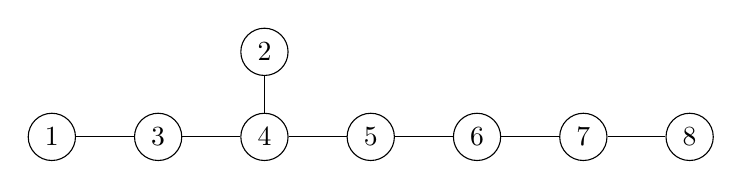
\begin{tikzpicture}[scale=0.9,
    every node/.style={circle, draw, fill=white, inner sep=2pt, minimum size=6mm}]
    
    % Nodes
    \node (1) at (0,0)   {$1$};
    \node (2) at (1.5,0) {$3$};
    \node (3) at (3,0)   {$4$};
    \node (4) at (4.5,0) {$5$};
    \node (5) at (6,0)   {$6$};
    \node (6) at (7.5,0) {$7$};
    \node (7) at (9,0)   {$8$};
    \node (8) at (3,1.2) {$2$};

    % Edges
    \draw (1)--(2)--(3)--(4)--(5)--(6)--(7);
    \draw (3)--(8);
\end{tikzpicture}
\caption{Dynkin diagram of $E_8$}
\end{figure}